\documentclass[pageno]{jpaper}

\newcommand{\IWreport}{2017}
\newcommand{\quotes}[1]{``#1''}


\widowpenalty=9999

\usepackage[normalem]{ulem}
\usepackage{graphicx}
\graphicspath{ {figures/} }


\begin{document}

\title{
Drone Based Measurement of Signal Propagation in Urban Environments and Analysis}

\author{Pranav Badami\\Adviser: Kyle Jamieson}

\date{}
\maketitle

\thispagestyle{empty}
\doublespacing

\begin{abstract}
ABSTRACT PLACEHOLDER
\end{abstract}

\section{Introduction (In Progress)}
\subsection{The Problem: ISP Monopolies in the United States}
Home Internet users in the United States are at the mercy of their Internet Service Provider(ISP). Users seeking relatively modern download (> 25 Mbps) and upload (> 3 Mbps) speeds for home Internet are extremely restricted in their choices. The FCC states that 30\% of Americans (measured in developed census blocks) have no ISPs delivering home Internet at these speeds, while another 48\% of Americans have only one ISP providing service at these speeds\cite{fcc15}. 

As a result of this lack of choice (and competition), American home Internet are forced to pay disproportionately high prices for relatively slow connections. For example, Americans pay higher prices for home Internet than Europeans across all categories of broadband speed[cite connectivity]:

INSERT FIGURE

The plight of the American home Internet user is exposed even more when considering the highest available home Internet speeds for affordable Internet plans. While residents of Seoul and Hong Kong can choose among plans offering 300 Mbps connections in the price range of \$35-\$50, no American city has any plans offering > 50 Mbps speeds for the same price range. [cite connectivity] The much cheaper and faster connections available in Asia demonstrate that it is technologically feasible to provide fast home Internet connections for a low price. 

Not coincidentally, ISPs in Asia operate in a much more competitive landscape, forcing them to provide quality service at a lower price. In South Korea, for example, upstart ISPs can lease, and sell, unused bandwidth from a public utility that reaches the vast majority of the clustered, urban population. Further, the South Korean government forced Korea Telecom to open its network in the '90s, leading to increased competition and lower prices for users[cite wired]. 

The competitive landscape of Home internet service in the United States is dramatically different for a few reasons. First, the FCC has not taken as drastic action to spur competition as government entities in Asia have. In 2014, Tom Wheeler, Chairman of the FCC, acknowledged the lack of competition among ISPs and recognized a need for the FCC to do more to protect and create competition in the United States [cite Wheeler]. The policy aspects of ISP competition are an entirely separate issue that will not be tackled here. 

Secondly, the population of the United States is large and spread out over a vast expanse of land. Reaching more homes in the United States requires laying lots of costly wire, which is often prohibitively expensive. Consider the efforts of Google Fiber. Google Fiber aims to offer connection speeds of 1000 Mbps at a comparable price to existing plans, reaching consumers in select neighborhoods of select American cities[cite google fiber]. According to Google, the process of bringing Fiber to a city involves initial exploration, network design, construction (laying fiber), and finally, customer sign up and installation. A Goldman Sachs report on Fiber, estimated that it would cost around \$140 billion for Google to cover the whole country[cite Goldman]. Further, the involved process required to dig and install fiber is extremely time consuming. The cost and time required to lay fiber across a wide geographic area makes it extremely difficult for even established companies like Google to enter the ISP realm, much less a host of smaller companies or startups.
\subsection{A (Potential) Solution: Wireless Mesh Networks}
With the cost of establishing novel, last-mile wired networks being so high, there has been a lot of work on establishing wireless networks. One such notable project is Roofnet, a wireless mesh featuring over 40 nodes spread out over the urban area of Cambridge, Massachusetts. Roofnet nodes consist of a small PC, an 802.11b card, and an 8 dBi omni-directional antenna. These nodes are primarily installed on three to four story tall buildings, with packets hopping wireless nodes until they reach a wireless node which is also connected to a gateway to the rest of the wired Internet[cite roofnet]. Individual users install these nodes on their roofs or windows and join the network. 

Similar to Roofnet, another community powered mesh exists in Red Hook, Brooklyn[cite NYT Red Hook]. The goal of these networks is to provide a cheaper, more accessible form of Internet architecture in comparison to the extremely expensive deployment of fiber cables. However, these wireless networks face challenges operating in the urban environment.

\subsection{Challenges with Wireless: Propagation and Measurement}
The propagation of wireless signals in a noisy, obstacle-ridden urban environment often results in wireless networks operating below peak efficiency. Buildings and other environmental obstacles, such as trees, can greatly increase the path loss of a wireless link between two nodes. Then, establishing a line-of-sight (LOS) connection between two wireless links is important for low-loss links and robust wireless networks. However, the Fresnel Zone (an ellipsoid-shaped volume) around the LOS must also be clear of obstacles for optimally low path loss between a transmitter and receiver. 
Much work has been conducted on measurement campaigns of wireless signal propagation. Theodore S. Rapaport has conducted many such campaigns in a variety of settings in order to explore real-world propagation in different environments. For example, Rapaport, Durgin, and Xu's "Measurements and Models for Radio Path Loss and Penetration Loss In and Around Homes and Trees at 5.8GHz" conducted such a campaign in a suburban area. Signal strength measurement were taken by moving a receiver around a 1m square area and averaged to represent the path loss for a given room or outdoor location[cite Rappaport]. Such campaigns, while useful for sampling signal strength at key locations, don't give a complete understanding of signal strength over a space. 
Other campaigns have attempted to get a more complete measurement in an urban environment. A group of Brazilian researchers conducted a measurement campaign in Rio De Janeiro with a fixed transmitter on the window of an 8 story building. They built a receiver block with GPS and collected measurements by driving around streets surrounding the building housing the transmitter. GPS and signal strength measurements collected by the receiver block are joined to construct a map of measured signal strength at street level. While this may be useful for mobile Internet users at the street level, participants in a wireless mesh for home Internet may have receiver nodes at various heights, necessitating a more 3-D measurement of signal propagation in urban areas. 
\subsection{[THIS PROJECT]: Robust Measurement}
This project aims to develop a novel, robust measurement technique to measure signal propagation in urban environments. Specifically, we aim to develop a technique that will provide a complete picture of signal propagation in 3-dimensional space around urban features. This is motivated by the desire to identify favorable locations for wireless mesh network nodes in cities and suburbs. \\
To do this, we will conduct a drone based wireless signal propagation measurement campaign in a handful of locations on the Princeton campus. A measurement apparatus collecting measurements across the 2.4GHz wireless spectrum and a GPS antenna will be mounted on a drone, which will collect measurements at varying heights. The collected data can then be aggregated to get a comprehensive, robust 3-dimensional map of signal strengths around a certain urban feature, such as a courtyard or a street with buildings on both sides. \\

The main research goal of this project is to be able to construct a plot of 3-D  "buckets" where the value associated with each bucket is the average signal strength measurement at a given frequency collected in the space occupied by that bucket. Fig 1 illustrates what such a plot may look like. A secondary research goal is to analyze these buckets of averaged values and determine which urban features led to higher overall signal strength. \\

This approach is novel because it yields a comprehensive, 3-Dimensional understanding of signal strength; existing measurement techniques are restricted to 2-Dimensional maps or point measurements. Since this project is motivated by wireless mesh networks,conducting measurements at various heights is important as users can be situated at various floors. Another benefit of this novel approach is the ability to potentially automate this measurement procedure for larger urban environments in the future. \\

\begin{figure}[h]
	\caption{A mockup of the primary research goal: constructing a plot of 3-D "buckets" representing signal strength around urban features (gray buildings) given a fixed position transmitter (white).}
	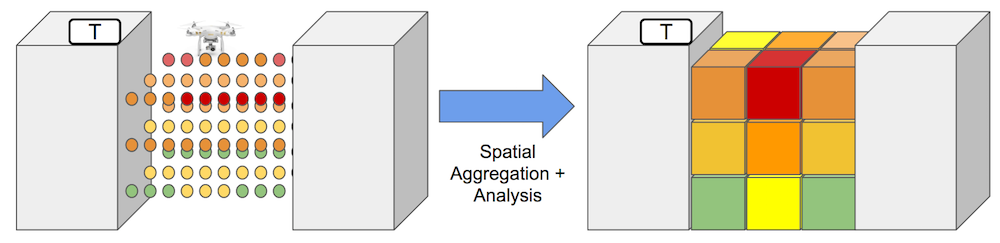
\includegraphics{measurement_goal}e
	\centering
\end{figure}


\section{Outline}  

\subsection{Introduction}
\begin{itemize}
	\item Motivation - What is the problem? Why is it important?
	\item Goal - What are we trying to accomplish?
	\item Overview of challenge and previous work 
	\item Approach 
	\item Summary of implementation
	\item Summary of results
	\item (optional) Roadmap: The remainder of this paper is organized as follows....
\end{itemize}

\subsection{Problem Background and Related Work}
\begin{itemize}
	\item Survey of prior work with similar goals 
	\item For each previous approach, explain what has been done and why it does not meet your goal
\end{itemize}

\subsection{Approach}
\begin{itemize}
	\item Key novel idea
	\item Why it is a good idea
\end{itemize}

\subsection{Implementation}
\begin{itemize}
	\item System overview (flow chart of key steps?)
	\item Subsection for each step or issue you addressed
	\begin{itemize}
		\item Problem statement
		\item Possible approaches
		\item Chosen approach and why
		\item Implementaton details
	\end{itemize}
\end{itemize}

\subsection{Evaluation}
\begin{itemize}
	\item Experiment design...
	\item Data...
	\item Metrics...
	\item Comparisons...
	\item Qualitative results...
	\item Quantitative results...
\end{itemize}

\subsection{Summary}
\begin{itemize}
	\item Conclusions...
	\item Limitations...
	\item Future work...
\end{itemize}



\bstctlcite{bstctl:etal, bstctl:nodash, bstctl:simpurl}
\bibliographystyle{IEEEtranS}
\bibliography{references}



\section{TEMPLATE REFERENCE: KAJ IGNORE}
\section{Preparation Instructions}

\subsection{Paper Formatting}
\label{section:formatting}

There are no minimum or maximum length limits on IW reports.  
We are including this template because we think it will be helpful
for citing things properly and for including figures into formatted
text.  If you are using \LaTeX~\cite{lamport94} 
to typeset your paper, then we strongly suggest
that you start from the template available at
http://iw.cs.princeton.edu -- this
document was prepared with that template.  
If you are using a different software package to typeset your paper, 
then you can still use this document as a reasonable sample of 
how your report might look.  Table~\ref{table:formatting} is a suggestion
of some formatting guidelines, as well as being an example of how to
include a table in a Latex document.

\begin{table}[hbt]
	\centering
	\begin{tabular}{|l|l|}
		\hline
		\textbf{Field} & \textbf{Value}\\
		\hline
		\hline
		Paper size & US Letter 8.5in $\times$ 11in\\
		\hline
		Top margin & 1in\\
		\hline
		Bottom margin & 1in\\
		\hline
		Left margin & 1in\\
		\hline
		Right margin & 1in\\
		\hline
		Body font & 12pt\\
		\hline
		Abstract font & 12pt, italicized\\
		\hline
		Section heading font & 14pt, bold\\
		\hline
		Subsection heading font & 12pt, bold\\
		\hline
	\end{tabular}
	\caption{Formatting guidelines. }
	\label{table:formatting}
\end{table}

\textbf{Please ensure that you include page numbers with your
	submission}. This makes it easier for readers to refer to
different parts of your paper when they provide comments.

We highly recommend you use bibtex for managing your references and citations.  You can add bib entries to a references.bib file throughout the semester (e.g., as you read papers) and then they will be ready for you to cite when you start writing the report.  If you use bibtex, please note that the references.bib file provided in the template example includes some format-specific incantations at the top of the file.  If you substitute your own bib file, you will probably want to include these 
incantations at the top of it.

\subsection{Citations and Footnotes}

There are various reasons to cite prior work and include it as references in your bibliography.  For example, If you are improving upon 
prior work, you should include
a full citation for the work in the bibliography \cite{nicepaper,nicepaper2}. 
You can also cite information that is used as background or
explanation\cite{Salzberg:2005}.  In addition to citing scholarly papers or books, you can
also create bibtex entries for webpages or other sources.  Many online
databases allow you to download a premade bibtex entry for each paper
you access.  You can simply copy-paste these into your references.bib
file.

Sometimes you want to footnote something, such as a web
site.\footnote{http://www.cs.princeton.edu}  Note that the footnote
number comes after the punctuation.

\subsection{Figures and Tables.}

Figure \ref{fig:gray} shows an example of how to include a figure in
your report.  
Ensure that the figures and
tables are legible.  Please also ensure that you refer to your
figures in the main text. Make sure that your figures will be legible
in the expected forms that the report will be read.  If you expect someone
to print it out in gray-scale, then make sure the figures are legible 
when printed that way.  

\begin{figure}[hbt]
	\centering
	
\includegraphics[width=0.75\linewidth]{gray.jpg}
	\caption{This is a gray image.}
	\label{fig:gray}
\end{figure}

In Section~\ref{section:formatting}, an example of a table was given.
(Note that the ``S'' in Section is capitalized.  Here's one more
example - see Table~\ref{table:data}.

\begin{table}[hbt]
	\centering
	\begin{tabular}{|l|l|} \hline
		\textbf{Some field} & \textbf{Another field}\\\hline
		200          &  10000 \\ \hline 
		400          &  20000 \\ \hline 
		800          &  40000 \\ \hline 
		1600        &  80000 \\ \hline 
		3200        &  160000 \\ \hline 
		6400        &  320000 \\ \hline 
	\end{tabular}
	\caption{Some data in a table. }
	\label{table:data}
\end{table}


Here's an example that shows how you can have side-by-side figures -
see Figure~\ref{fig:side-a} and Figure~\ref{fig:side-b}.  (Note that
the the ``F'' in Figure is capitalized. 

\begin{figure}[htbb]
	\begin{minipage}[b]{0.5\linewidth}
		\centering
		
\includegraphics[width=.75\linewidth]{checkerboard-squares-black-white.jpg}
		\caption{Plain checkerboard.}
		\label{fig:side-a}
	\end{minipage}
	\hspace{0.5cm}
	\begin{minipage}[b]{0.5\linewidth}
		\centering
		
\includegraphics[width=.75\linewidth]{swirl-squares-black-white.jpg}
		\caption{Cool checkerboard.}
		\label{fig:side-b}
	\end{minipage}
\end{figure}

\subsection{Double Quotes.}

Latex double quotes are not the same as the double quote key on your
keyboard. The standard way of writing quotes and double quotes in
LaTeX is with `` and '' not with " and ".   

Now that may be confusing, so you may want to use the \textbackslash\{quotes\} command.  For
example \quotes{The quick brown fox.}



\subsection{Main Body.}

Avoid bad page or column breaks in
your main text, i.e., last line of a paragraph at the top of a
column or first line of a paragraph at the end of a column. If you
begin a new section or sub-section near the end of a column,
ensure that you have at least two (2)  lines of body text on the same
column. 





\end{document}

